\documentclass[article,10pt]{scrartcl}
\usepackage{graphicx}
\usepackage{amsmath}
\usepackage{tikz}
\usepackage{vmargin}
\setmarginsrb{1.3cm}{1.3cm}{1.3cm}{1.3cm}{1.3cm}{1.3cm}{1.3cm}{1.3cm}
\setlength{\parindent}{0cm}
\usepackage{color}
\usepackage{listings}
\usepackage{hyperref}


\hypersetup{
    bookmarks=true,         % show bookmarks bar?
    unicode=false,          % non-Latin characters in Acrobat’s bookmarks
    pdftoolbar=true,        % show Acrobat’s toolbar?
    pdfmenubar=true,        % show Acrobat’s menu?
    pdffitwindow=false,     % window fit to page when opened
    pdfstartview={FitH},    % fits the width of the page to the window
    pdfnewwindow=true,      % links in new window
    colorlinks=true,       % false: boxed links; true: colored links
    linkcolor=black,          % color of internal links (change box color with linkbordercolor)
    citecolor=black,        % color of links to bibliography
    filecolor=black,      % color of file links
    urlcolor=black           % color of external links
}


\usepackage[final]{pdfpages}
% python script syntax taken from 
% http://widerin.org/blog/syntax-highlighting-for-python-scripts-in-latex-documents
\definecolor{Code}{rgb}{0,0,0}
\definecolor{Decorators}{rgb}{0.5,0.5,0.5}
\definecolor{Numbers}{rgb}{0.5,0,0}
\definecolor{MatchingBrackets}{rgb}{0.25,0.5,0.5}
\definecolor{Keywords}{rgb}{0,0,1}
\definecolor{self}{rgb}{0,0,0}
\definecolor{Strings}{rgb}{0,0.63,0}
\definecolor{Comments}{rgb}{0,0.63,1}
\definecolor{Backquotes}{rgb}{0,0,0}
\definecolor{Classname}{rgb}{0,0,0}
\definecolor{FunctionName}{rgb}{0,0,0}
\definecolor{Operators}{rgb}{0,0,0}
\definecolor{Background}{rgb}{0.98,0.98,0.98}

\lstnewenvironment{python}[1][]{
\lstset{
%numbers=left,
%numberstyle=\footnotesize,
%numbersep=1em,
xleftmargin=1em,
framextopmargin=2em,
framexbottommargin=2em,
showspaces=false,
showtabs=false,
showstringspaces=false,
frame=l,
tabsize=3,
% Basic
%basicstyle=\ttfamily\small\setstretch{},
backgroundcolor=\color{Background},
language=Python,
% Comments
commentstyle=\color{Comments}\slshape,
% Strings
stringstyle=\color{Strings},
morecomment=[s][\color{Strings}]{"""}{"""},
morecomment=[s][\color{Strings}]{'''}{'''},
% keywords
morekeywords={import,from,class,def,for,while,if,is,in,elif,else,not,and,or,print,break,continue,return,True,False,None,access,as,,del,except,exec,finally,global,import,lambda,pass,print,raise,try,assert},
keywordstyle={\color{Keywords}\bfseries},
% additional keywords
morekeywords={[2]@invariant},
keywordstyle={[2]\color{Decorators}\slshape},
emph={self},
emphstyle={\color{self}\slshape},
%
}}{}

\begin{document}
\title{Read and Plot data with Python}
\subtitle{Student and Staff IT Introduction}
\maketitle

\section{Read data from a .CSV file}

\paragraph{}
There is different ways to open and read a CSV (Comma Separated Values) file in python. You can export the Excel spreadsheets into CSV. Here is the easiest way using only the standard libraries of Python.
The CSV file here contains only one column with float numbers. Try the following code on file ``csv1.csv'':

\begin{python}
import sys

# sys.argv is a list containing the command line parameters
# sys.argv[0] always contains the name of the python script
if len(sys.argv) != 2:
   print 'Error: give a file name on the command line'
   exit(1) # Exit and return the error code 1

csv_file_name = sys.argv[1]
csv = open(csv_file_name, 'r') #open the csv file
data = [] #initiation of the data list
for line in csv: #read the file
   line = line.rstrip() # remove the 'newline' character at the end of the line
   data.append(float(line))#append the current value in the data list
print data
csv.close() #close the csv file
\end{python}

\paragraph{}
It can be a bit harder to read files containing many columns and/or column lines, but hopefully, there is python libraries allowing to read csv files. Here we will use a function call ``\emph{genfromtxt}'' from the library \emph{numpy}. Try to open the file ``csv2.csv'' using the following code. The file contains two columns of values. The first row of the file correspond to the names of the columns: ``V1'' and ``V2''. To load data from a CSV file using ``genfromtxt'', you have to specify a delimiter (the comma here), the type of your data (not mandatory). If columns names are present in the file, you should use the ``skip\_header'' option.
\paragraph{}

\begin{python}
import sys
import numpy as np

if len(sys.argv) != 2:
   print 'Error: give a file name on the command line'
   exit(1) # Exit and return the error code 1

data = np.genfromtxt(sys.argv[1], dtype=float, delimiter=',', skip_header=True) 

print data # All data
print data[:,0] # column 1
print data[:,1] # column 2

\end{python}
\paragraph{}
You can find more information about the function options ``genfromtxt'' of numpy here: \url{http://docs.scipy.org/doc/numpy/user/basics.io.genfromtxt.html}. The ``names'' option might be interesting to work on columns only. You can find a tutorial about another library allowing to read and write CSV files here: \url{http://www.pythonforbeginners.com/systems-programming/using-the-csv-module-in-python/}
Now you know how to read data from a simple text file, so lets see how to plot these data.

\section{Scatter Plot}
\paragraph{}
To plot the data we will use the \emph{pyplot} module from \emph{matplotlib} library. We will modify the code we used to read the simple CSV file (csv1.csv) to plot the data.
\paragraph{}
\begin{python}
import matplotlib.pyplot as plt # import the pyplot module as plt
import sys

# sys.argv is a list containing the command line parameters
# sys.argv[0] always contains the name of the python script
if len(sys.argv) != 2:
   print 'Error: give a file name on the command line'
   exit(1) # Exit and return the error code 1

csv_file_name = sys.argv[1]
csv = open(csv_file_name, 'r') #open the csv file
data = [] #initiation of the data list
for line in csv: #read the file
   line = line.rstrip() # remove the 'newline' character at the end of the line
   data.append(float(line))#append the current value in the data list
print data
csv.close() #close the csv file

plt.plot(data) #Simple scatter plot of the data
plt.ylabel('My data') #title of the Y axis
plt.show() # show the plot
\end{python}
\paragraph{}
The default values for the X axis are a simple ``range(N)'', but it is possible to set these values using the same ``plot'' function. Here is a simple example:
\paragraph{}
\begin{python}
x = [1, 2, 3, 4, 5, 6]
y = [1, 2, 4, 3, 6, 5]  
plt.plot( x, y )
plt.xlabel( "X values" )
plt.ylabel( "Y values" )
plt.show()
\end{python}
\paragraph{}
\emph{Exercise}: Try to build a script to plot the data of the file ``csv2.csv''.
You should obtain a graphic like:
\begin{figure}[h!]
\begin{center}
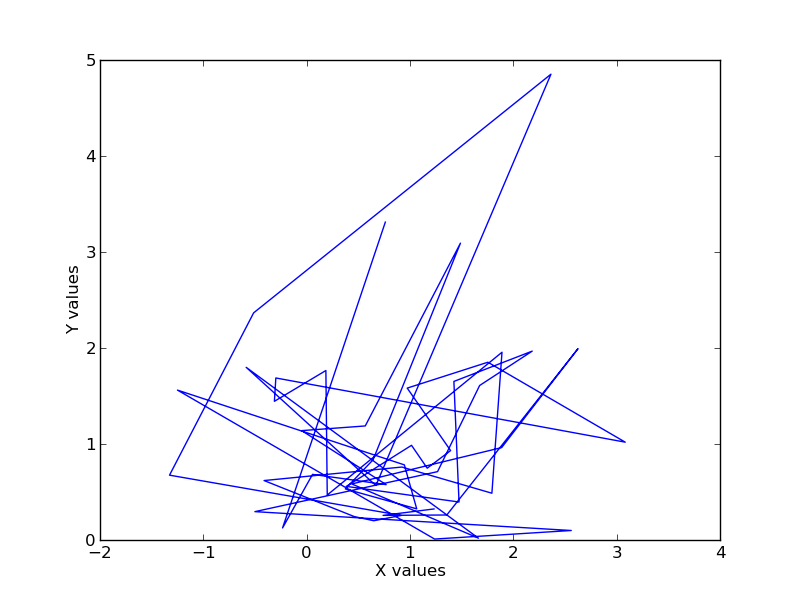
\includegraphics[scale=0.5]{figure_1.png}\\
\end{center}
\end{figure}
\paragraph{}
These data points shouldn't be linked by lines in the plot. Here is an example showing how to configure the plot displays:
\paragraph{}
\begin{python}
import numpy as np
import matplotlib.pyplot as plt

# evenly sampled time at 200ms intervals
t = np.arange(0., 5., 0.2) #Simple data data. Same as range() function

# red dashes, blue squares and green triangles
plt.plot(t, t, 'r--')    #Red (r) dashes (--)
plt.plot(t, t**2, 'bs')  #Blue (b) squares (s)
plt.plot(t, t**3, 'g^')  #Green (g) triangles (^)
plt.plot(t, t**4, 'b+-') #Blue (b) crosses (+) linked by a line (-)
plt.show()
\end{python}
\paragraph{}
Using this example, change your script to display the data using independent blue dots. The different markers are: 
\begin{python}
[ 7  |  4  |   5    |   6  | 'o' | 'D' | 
 '_' | ''  | 'None' | None | ' ' | '8' | 
 'p' | ',' |  '+'   |  '.' | 's' | '*' | 
 3   |  0  |   1    |   2  | '1' | '3' | 
 'v' | '<' |  '>'   |  '^' | '|' | 'x' |
 'h' | 'H' |  'd'   |  '4' | '2' ]
\end{python}
\paragraph{}
The different line styles are:
\begin{python}
[ '-' | '--' | '-.' | ':' | 'None' | ' ' | '' ] 
\end{python}
\paragraph{}
Now you know how to build line plots and scatter plots, lets see how to build box plots.

\section{Box plot}
\paragraph{}
Here is an example of code building a box plot from random data. Try it, then display the values of the file ``cvs3.csv'' using a box plot. 
\paragraph{}
\begin{python}
import matplotlib.pyplot as plt
import numpy as np

#Fake data generation (random position on a normal law)
e1 = np.random.normal(0, 1, size=(500,))
e2 = np.random.normal(0, 1, size=(500,))
e3 = np.random.normal(0, 2, size=(500,))
e4 = np.random.normal(0, 2, size=(500,))

data=[e1,e2,e3,e4]
plt.boxplot(data)
plt.show()
\end{python}
\paragraph{}
The ``plt.boxplot'' function makes a box and whisker plot for each column of the given data.  The box extends from the lower to upper quartile values of the data, with a line at the median.
The whiskers extend from the box to show the range of the data.  The length of the whiskers is defined as a function of the inner quartile range (by default 1.5 times longer). Flier points are those past the end of the whiskers. 
\paragraph{}
\emph{Remarks}: PyPlot allows you to specify your own values for the confidence interval, the whiskers length  and the median.

\section{More resources}
You can find many resources online for python, numpy and matplotlib
\begin{itemize}
\item There is a good introdution to NumPy and Matplotlib for python beginners here: \url{http://youtu.be/3Fp1zn5ao2M}
\item A NumPy tutorial on SciPy website: \url{http://wiki.scipy.org/Tentative_NumPy_Tutorial}
\item A Matplotlib tutorial on SciPy website: \url{http://wiki.scipy.org/Cookbook/Matplotlib/}
\item Matplotlib documentation is really good, it contains also a lot of examples and tutorials: \url{http://matplotlib.org}
\item A tutorial with a lot of styling options: \url{http://cs.smith.edu/dftwiki/index.php/MatPlotLib_Tutorial_1}
\item Another really good introduction to most of the plot types available in Matplotlib: \url{http://www.loria.fr/~rougier/teaching/matplotlib/}
\end{itemize}

\end{document}
